\documentclass[conference]{IEEEtran}
%+++++++++++++++++++++++++++++++++++++++++++
% Added to commands
\input epsf
\usepackage{graphicx}
\usepackage [french]{babel}
\usepackage [utf8]{inputenc}
\usepackage [T1] {fontenc}
\usepackage{float}
%+++++++++++++++++++++++++++++++++++++++++++
% correct bad hyphenation here
\hyphenation{op-tical net-works semi-conduc-tor IEEEtran}
\begin{document}

%+++++++++++++++++++++++++++++++++++++++++++
\title{\LARGE Etude de l'influence du diamètre et de la profondeur sur la finesse d'un kite
\vskip10pt

\small 2024 - Romain LAMBERT
}
%+++++++++++++++++++++++++++++++++++++++++++
% make the title area
\maketitle

\begin{abstract}Ce bureau d'étude a pour sujet l'étude de l'influence du \textbf{diamètre} (diameter) et de la \textbf{cambrure} (depth) sur la finesse d'un kite. L'objectif final étant de déterminer un couple (t,k) = (diameter, depth) qui serve de référence pour le dimensionnement des kites. Aussi, cette étude permet d'évaluer la sensibilité de la \textbf{VSM} sous la théorie 2D de la \textbf{regression de Breukels} à ces deux paramètres.
\end{abstract}
\IEEEoverridecommandlockouts

\IEEEpeerreviewmaketitle
\section{La théorie}

\subsection{\textbf{Regresion de Breukels : théorie 2D}} 

Si la VSM permet d'étudier l'aérodynamique 3D d'un kite, elle requiert le calcul des coefficients 2D de chaque section($C_L$, $C_D$, $C_M$). Afin de limiter le coût de calcul et de se baser sur des polaires adaptées à des profils "non conventionnels", la VSM utilise une \underline{formule de regression de Breukels}. 
Cette formule est issue de résultats obtenus sur des profils typiques de kites à boudin, et ne \underline{dépend que du diamètre du boudin et de la cambrure du profil}. \\


\begin{center}
    \begin{equation}
        C_L = \lambda_5  \alpha^3 +\lambda_6  \alpha^2 + \lambda_7  \alpha + \lambda_8
        \label{eq:Cl_breukels}
    \end{equation}
\end{center}
avec :
\begin{center}
    \begin{equation}
        \lambda_i = S_x  k + S_y
        \label{eq:lamba_breukels}
    \end{equation}
\end{center}
et :
\begin{center}
    \begin{equation}
        S_i = C_x  t^2 + C_y  t + C_z
        \label{eq:S_breukels}
    \end{equation}
\end{center}
où les 23 coéfficients $C_x$ sont prédéterminés, et (t,k) est le couple (diamètre, cambrure) définit tel que :
\begin{center}
    \begin{equation}
        t = \frac{Diamètre_{BA}}{Corde} ; k = \frac{max(CoordonéesExtrados)}{Corde}
        \label{eq:tk_breukels}
    \end{equation}
\end{center}

Ainsi, l'obtention ds coéfficients 2D permet ensuite à la VSM d'ajouter l'indluence des effets 3D (loi de corde, d'envergure, de voute...) sur les coefficients aérodynamique d'un kite

%%%%%%%%%%%%%%%%%%%%%%%%%%%%%%%%%%%%%%%%%%%%%%%%%%%%%%%%%%%%%%%%%%%%%%%%%
\IEEEpeerreviewmaketitle
\section{Le Code }

\subsection{Le cas d'étude - 2D} 

On étudie dans un premier temps La fonction de Breukels pour en chercher les optimum. On utilise pour ce faire un code d'optimsiation fournit par la bibliothèque \textbf{aerosandbox} et on se place dans deux cas d'optimisation : 
\begin{itemize}
    \item Maximum de $\frac{C_L(\alpha)}{C_D(\alpha)}$ à angle $\alpha$ fixé 
    \item Maximum de $\sum_{\alpha = 0}^{21}\frac{C_L(\alpha)}{C_D(\alpha)} Gaussienne(alpha, center, sigma) $
\end{itemize}

    où $Gaussienne(\alpha, center, \sigma) = e^{-\frac{(center - \alpha)^2}{2\sigma^2}}$ est une Gaussienne permettant d'obtenir une moyenne pondérée. 

\textbf{Pour notre étude, on choisit Center = 7° et sigma = 8}. Les résultats sont présentés dans la partie suivante.
\begin{figure}[H]
    \centering
    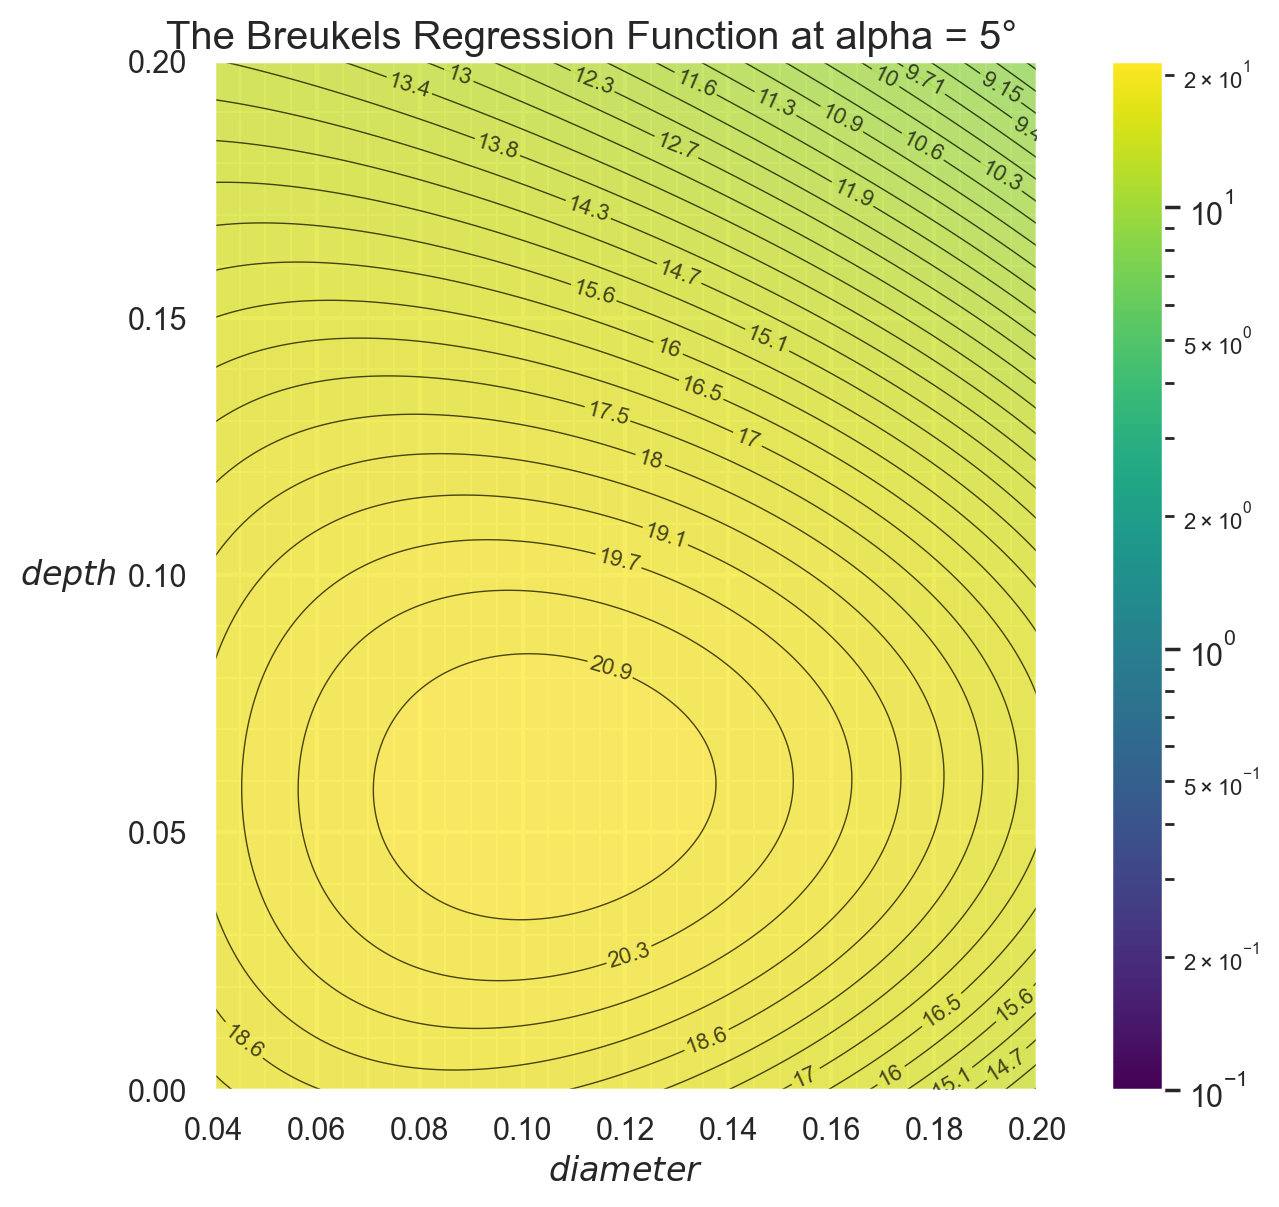
\includegraphics[width=0.5\textwidth]{Pics/breukels.png}  
    \caption{Tracer de $\frac{C_L}{C_D}$ par Régression de Breukels à $\alpha$=5°}
    \label{fig:breukels}
\end{figure}


\subsection{Le cas d'étude - 3D} 

On se place ensuite dans le cas d'étude d'un SK50-VG dont on fait varier le \textbf{diamètre t entre -0.02 et +0.1 et la cambrure k entre -0.1 et 0.1}. A noter que sur chaque section de l'aile \textbf{le diamètre ne peut pas être inférieur à 0.04 et la cambrure inférieur au demi-diamètre}. Ainsi, les résultats sont à nuancer : \textbf{une aile avec un delta de t ou de k ne veut as dire que toutes les sections ont été modifiées de ce delta}; seules les sections respectant ces critères énoncés précédemment le sont.

La loi d'évolution de t et k sur une VG est initialement:  
\begin{itemize}
    \item t : [0.07 0.067 0.065 0.063 0.061 0.06 0.06  0.06 0.06 0.06  0.06  0.06 0.06 0.06  0.06 0.061 0.063 0.065 0.067 0.07]
    \item k : [0.034 0.05 0.0645 0.0686 0.072 0.075 0.08 0.08 0.08 0.08      0.08 0.08 0.08 0.08 0.075 0.072 0.0686 0.0645 0.05 0.034]
\end{itemize}

    A nouveau, on cherche l'optimum dans les 2 problèmes d'optimisation suivants:
    \begin{itemize}
        \item Maximum de $\frac{C_L(\alpha)}{C_D(\alpha)}$ à angle $\alpha$ fixé 
        \item Maximum de $\sum_{\alpha = 0}^{21}\frac{C_L(\alpha)}{C_D(\alpha)} Gaussienne(alpha, center, sigma) $
    \end{itemize}
    Les résultats sont présentés dans la partie suivante.

\begin{figure}[H]
    \centering
    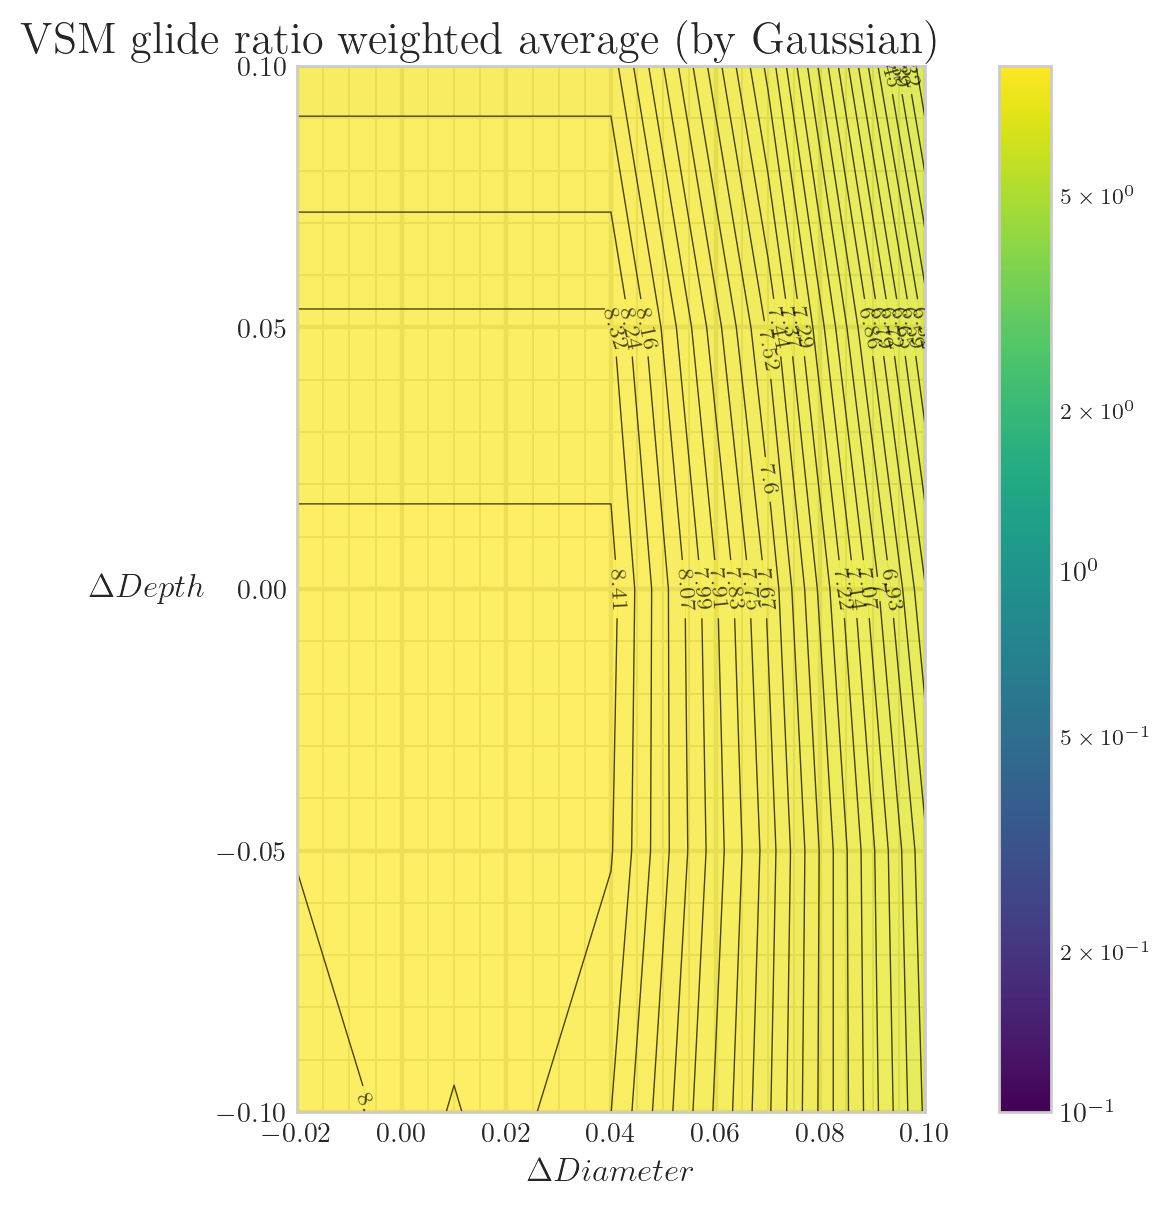
\includegraphics[width=0.5\textwidth]{Pics/vsm.png}  
    \caption{Tracer de $\frac{C_L}{C_D}$ par VSM en faisant varier (t,k)}
    \label{fig:vsm}
\end{figure}


%%%%%%%%%%%%%%%%%%%%%%%%%%%%%%%%%%%%%%%%%%%%%%%%%%%%%%%%%%%%%%%%%%%%%%%%%
\IEEEpeerreviewmaketitle
\section{Les Résultats}

\subsection{2D - résultats par $\alpha$}

\[
\begin{array}{|c|c|c|}
    \hline
    \textbf{$\alpha$} & \textbf{diamètre} & \textbf{cambrure}\\
    \hline
    0 & 0.040 & 0.20 \\
    1 & 0.091 & 0.00 \\
    2 & 0.098 & 0.00 \\
    3 & 0.10 & 0.01  \\
    4 & 0.10 & 0.04  \\
    5 & 0.10 & 0.06  \\
    6 & 0.10 & 0.068  \\
    7 & 0.095 & 0.074 \\
    8 & 0.089 & 0.078 \\
    9 & 0.079 & 0.082 \\
    10 & 0.061 & 0.086 \\
    11 & 0.040 & 0.093 \\
    12 & 0.040 & 0.103 \\
    13 & 0.040 & 0.105 \\
    14 & 0.040 & 0.107 \\
    15 & 0.040 & 0.109 \\
    16 & 0.040 & 0.111 \\
    17 & 0.040 & 0.113 \\
    18 & 0.040 & 0.115 \\
    19 & 0.040 & 0.118 \\
    20 & 0.040 & 0.121 \\
    \hline
\end{array}
\]

\begin{figure}[H]
    \centering
    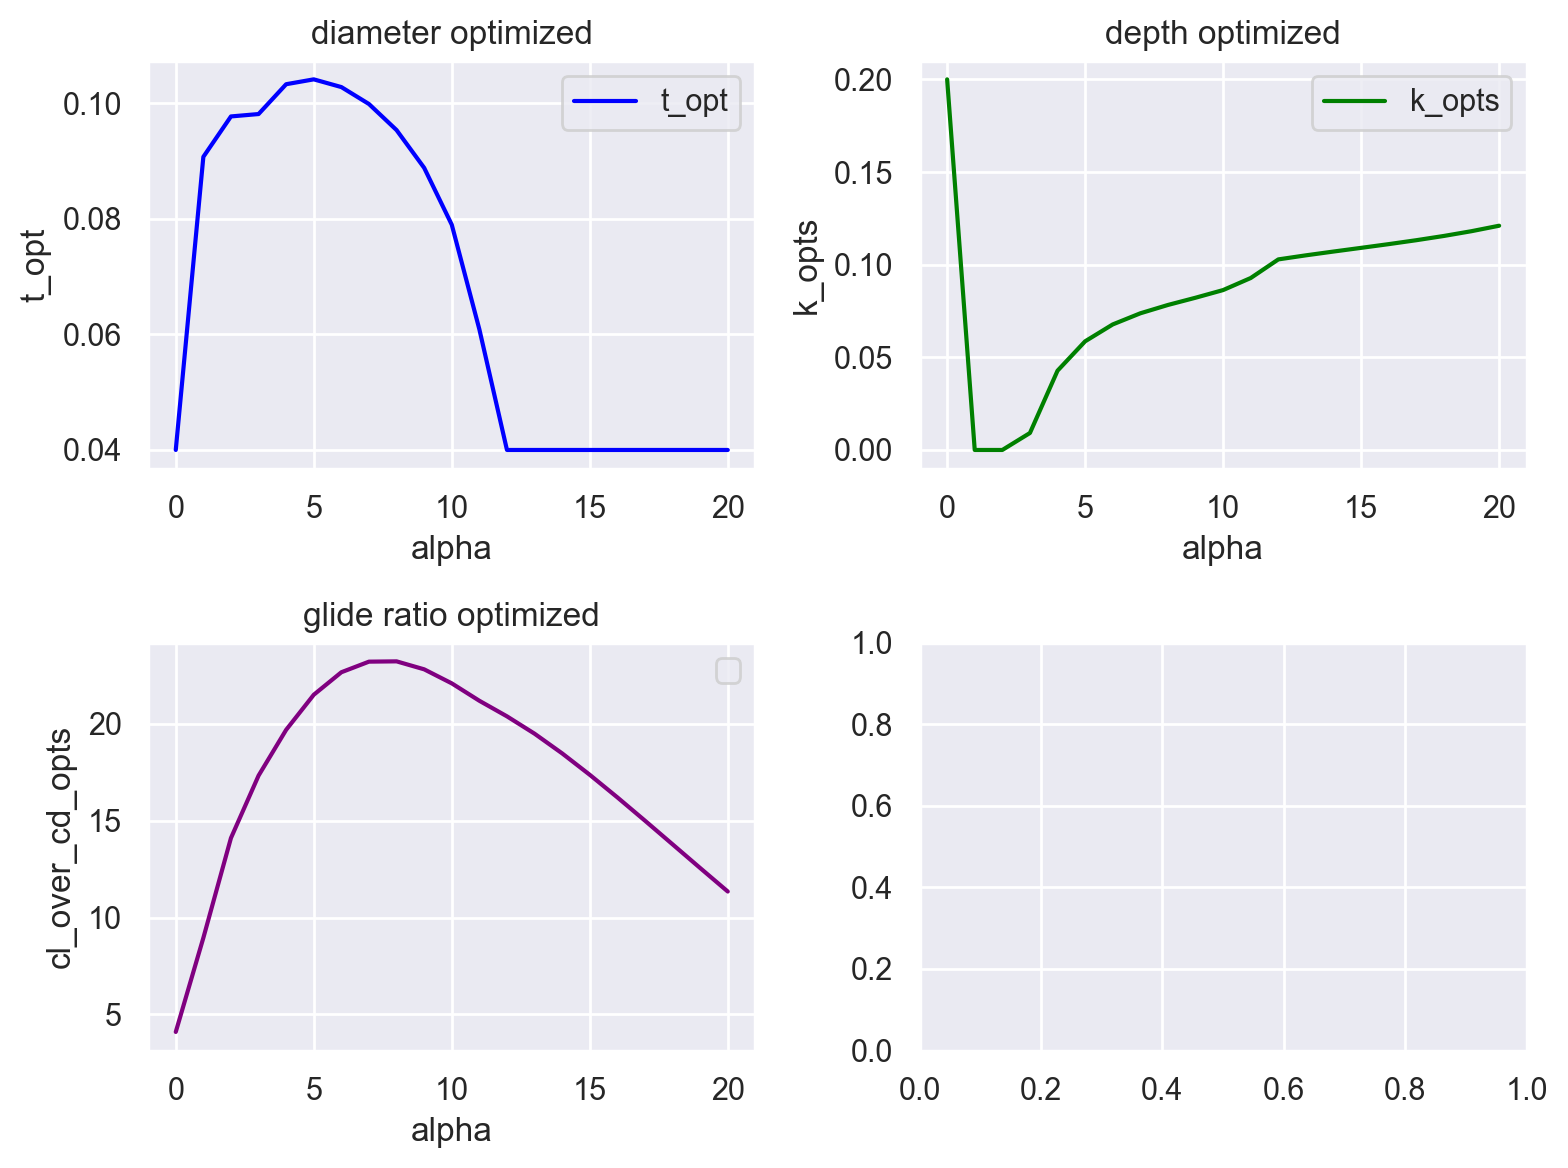
\includegraphics[width=0.5\textwidth]{Pics/résultats pas alpha 2D.png}  
    \caption{Tracer de t et k optimaux pour chaque alpha}
    \label{fig:t,k,alpha 2d}
\end{figure}

    \textbf{Remarque :} 
    \begin{itemize}
        \item On observe que pour les grands angles le diamètre optimal tend à être le plus petit possible.
        \item La cambrure optimale augmente avec $\alpha$.
        \item Les résultats sont cohérents en ordre de grandeur
    \end{itemize}

\subsection{2D - résultats avec moyenne pondérée par Gaussienne}

    Avec une Gaussienne de paramètres \textbf{center = 7° et sigma = 8}, les valeurs qui maximisent la fonction objective (moyenne pondérée de finesse aérodynamique) sont :
    \begin{itemize}
        \item t : 0.0745
        \item k : 0.0860
    \end{itemize}
    \textbf{Ces résultats sont cohérents en ordre de grandeur.}

\subsection{3D - résultats par $\alpha$}

\[
\begin{array}{|c|c|c|c|c|}
    \hline
    \textbf{$\alpha$} & \textbf{$\delta diametre$} & \textbf{nombre ribs saturés en diamètre} & \textbf{$\delta cambrure$} & \textbf{nombre ribs saturés en cambrure}\\
    \hline
    0 & -0.02 & 10 & -0.05 & 10\\
    1 & -0.02 & 10 & -0.05 & 10\\
    2 & -0.02 & 10 & -0.05 & 10\\
    3 & -0.02 & 10 & -0.05 & 10 \\
    4 & -0.02 & 10 & -0.05 & 10 \\
    5 & -0.02 & 10 & -0.05 & 10 \\
    6 & -0.02 & 10 & -0.05 & 10  \\
    7 & -0.02 & 10 & -0.05 & 10 \\
    8 & -0.02 & 10 & -0.05 & 10 \\
    9 & -0.02 & 10 & -0.05 & 10 \\
    10 & -0.02 & 10 & -0.05 & 10 \\
    11 & 0.04 & 0 & -0.1 & 20 \\
    12 & 0.04 & 0 & -0.1 & 20 \\
    13 & 0.04 & 0 & -0.1 & 20 \\
    14 & 0.04 & 0 & -0.1 & 20 \\
    15 & 0.01 & 0 & -0.1 & 20 \\
    16 & 0.01 & 0 & -0.1 & 20 \\
    17 & 0.01 & 0 & -0.1 & 20 \\
    18 & 0.01 & 0 & -0.1 & 20 \\
    19 & 0.01 & 0 & -0.1 & 20 \\
    20 & 0.01 & 0 & -0.1 & 20 \\
    \hline
\end{array}
\]
    \textbf{Remarque :}
    \begin{itemize}
        \item Pour beaucoup de valeurs optimales, un nombre importants de ribs sont saturés en cambrure et diamètre; c'est à dire qu'ils sont limités par la condition de valeurs minimale. \textbf{Ce sont les rib sur les tips qui saturent en premier}
        \item Le faible nombre d'échantillon semble limité la précision des résultats. Avec 5 valeurs de $\delta Diameter$ et 5 valeurs de $\delta Depth$, on est déjà à 5x5 = 25 simulations (10 minutes)!
    \end{itemize}

\subsection{3D - résultats avec moyenne pondérée par Gaussienne}
Avec une Gaussienne de paramètres \textbf{center = 7° et sigma = 8}, les valeurs qui maximisent la fonction objective (moyenne pondérée de finesse aérodynamique) sont :
\begin{itemize}
    \item $\delta diameter$ : -0.02
    \item $\delta depth$ : -0.05
\end{itemize}

\textbf{Les valeurs de diamètre et cambrure optimaux ainsi obtenus en 3D sont : 
}

\begin{itemize}
    \item t : 0.080 0.077 0.0757 0.073 0.0713 0.070 0.070  0.070 0.070 0.0709  0.070  0.070 0.070 0.070 0.070 0.071 0.073 0.075 0.077 0.080
    \item k : 0.040 0.038 0.038 0.036 0.035 0.035 0.035  0.035 0.035 0.035 0.035 0.035 0.035 0.035  0.035 0.035 0.036 0.038 0.038 0.040
\end{itemize}

\end{document}